\documentclass[tikz,border=3mm]{standalone}
\usepackage{amsmath}
\usetikzlibrary{intersections}
\begin{document}
	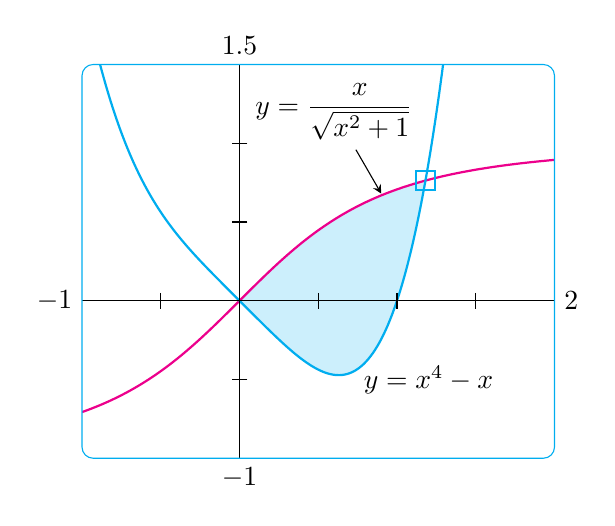
\begin{tikzpicture}[scale=2]
		\def\bb{[rounded corners] (-1,-1) rectangle (2,1.5)}
		\def\curveA{plot[domain=-1:2,smooth,samples=100]  (\x,{\x/(sqrt(1+\x*\x))})}
		\def\curveB{plot[domain=-1:2,smooth,samples=100](\x,{pow(\x,4)-\x})}
		\begin{scope} \clip \bb;
			\begin{scope} 
				\clip \curveA|-cycle;
				\clip \curveB--cycle;
				\fill[cyan!20] \bb;
			\end{scope}
			\draw (-1,0)--(2,0) (0,-1)--(0,1.5);
			\draw[magenta,thick,name path=A] \curveA;
			\draw[cyan,thick,name path=B] \curveB;
			\path[name intersections={of=A and B}] (intersection-2) node[cyan,rectangle,minimum size=2mm,draw,thick]{};
		\end{scope}
		\draw[cyan] \bb;
		\foreach \i in {-.5,0,...,1.5} \draw (\i,.05)--(\i,-.05);
		\foreach \j in {-.5,0,...,1} \draw (.05,\j)--(-.05,\j);
		\path
		(-1,0) node[left]{$-1$}
		(2,0) node[right]{$2$}
		(0,-1) node[below]{$-1$}
		(0,1.5) node[above]{$1.5$}
		(1.2,-.5) node{$y=x^4-x$}
		(.6,1.2) node (N) {$y=\dfrac{x}{\sqrt{x^2+1}}$};
		\draw[-stealth] (N)--+(-60:.6);
	\end{tikzpicture}
\end{document}